\documentclass[openany,justified]{tufte-book}

%% --- note that the file "tufte-book-local.tex" is also read

%% --- packages

\usepackage{graphicx}      %% figures
\usepackage{eag_names}     %% journal names
\usepackage{natbib}        %% citations
\usepackage{listings}
\usepackage{hyperref}

\usepackage[Bjornstrup]{fncychap}

\definecolor{gray}{rgb}{0.5,0.5,0.5}
\definecolor{lightgray}{rgb}{0.97,0.97,0.97}
\lstset{language=Python,
  aboveskip=4mm,
  belowskip=4mm,
  showstringspaces=false,
  columns=flexible,
  basicstyle={\footnotesize\ttfamily},
  numbers=none,
  backgroundcolor=\color{lightgray},
  numberstyle=\tiny\color{gray},
  keywordstyle=\color{gray},
  commentstyle=\color{gray},
  stringstyle=\color{gray},
  breaklines=true,
  breakatwhitespace=true,
  tabsize=4
}

%% --- start definitions

\graphicspath{{figures/}}  %% default path for figures

\title{EISPAC User's Guide}
\author[EIS Team]{EIS Team}

\def\arcsec{\hbox{$^{\prime\prime}$}}
\def\ion#1#2{#1\,{\sc\romannumeral #2}\relax}

%% --- end definitions

\begin{document}

\maketitle
\tableofcontents

%% --- the chapters


\chapter{Introduction}

\newthought{The EUV Imaging Spectrometer} --- EIS --- was designed to study the solar atmosphere and
answer fundamental questions on the heating of the solar corona, the origin of the solar wind, and the
release of energy in solar flares\sidenote{EIS is part of the Hinode mission and
  was sponsored by the Japan Aerospace Exploration Agency (JAXA), the United Kingdom Space Agency
  (UKSA), and National Aeronautics and Space Administration (NASA) with contributions from ESA and
  Norway. Hinode was launched on September 22, 2006 at 21:36 UTC from the Uchinoura Space Center in
  Japan and continues to operate.}. EIS observes two wavelength ranges in the extreme ultraviolet,
171–-212\,\AA\ and 245–-291\,\AA\ with a spectral resolution of about 22\,m\AA\ and a plate scale
of 1\arcsec\ per pixel. Solar images can be made by stepping the slit over a region of the Sun and
taking an exposure at each position. A detailed description of EIS is given in the instrument
paper\cite{Culhane:2007}.

This document describes the basic elements of EIS data analysis using new HDF5 level-1 files and
the EIS Python Analysis Code (EISPAC) package. At the beginning of the Hinode mission the
strategy was to release unprocessed level-0 FITS files and software routines written in IDL for
processing these files into a format that could be used for data analysis. Additionally, all of
the routines for computing ancillary information, such as the offsets of the detectors or the magnitude
of the instrumental broadening, were all written in IDL. Unfortunately, IDL is an expensive,
proprietary language, little used outside of solar physics. Python, in contrast, is a free, open
source language that has grown dramatically in popularity since the launch of Hinode, making it an
obvious choice for future software development.

\section{EIS Level-1 HDF5 Files}
To accelerate the transition to Python we have created a new level-1 product that contains both the
processed level-1 data and the ancillary information needed for data analysis. The alternative
approach, to port all of the existing IDL software to Python, would be time consuming and create
confusion about which routines are being actively supported during the transition. Distributing
level-1 files removes this problem, but does make the user dependent on the team for reformatting
all of the files as bugs are discovered. Since the mission has been going on for some time now, the
number of bugs is likely to be small.

There are several other design decisions that merit some explanation

\begin{itemize}
  \item The data and header information are stored in separate files. Since the data is large and
    unlikely to change, the time-consuming download of these files should only need to be done
    once. The header file is very small and can be updated easily.
  \item HDF5 is used to store the data. This is a very widely used, high-performance file format
    that is well supported by both IDL and Python. The most attractive feature for this application
    is that data is stored in a self-documenting, directory-like tree structure instead of binary
    table extensions.
  \item The data is processed from raw ``data numbers'' to ``photon events'' or ``counts''. The
    default behavior of \verb+eis_prep+ is to convert to calibrated units. With the HDF5 files
    conversion to absolute units is done using a calibration curve in the header file, and several
    different calibration curves can be considered.
\end{itemize}

The processed level-1 HDF5 files can be downloaded either directly from the NRL Hinode/EIS website at \url{https://eis.nrl.navy.mil/} or using the tools included in EISPAC. \hyperref[sec:prep]{Chapter 4} describes the processing of the files in more detail.

\section{EIS Python Analysis Code (EISPAC)}
EISPAC provides Python classes and functions that can read the new HDF5 files, perform all of the
necessary calibration and pointing adjustments, and create user-friendly Python objects that can be
manipulated as needed. Also included are functions for fitting the intensity profiles with multi-
Gaussian functions using template files and a Python port of the venerable \verb+MPFIT+ library
\citep{Markwardt:2009}. For convenience, command line and GUI tools are provided to help users quickly
browse and download data, copy template files, and fit multiple files at once using parallel
processing.

\subsection{Requirements}
EISPAC depends on a number of Python packages that are commonly used in scientific and solar research.
Normally, the installation process should automatically check and install missing dependencies,
assuming your environment is configured appropriately. If it does not, you may wish to try installing
the required packages individually first.
\begin{itemize}
    \item python >= 3.7
    \item numpy >= 1.18.1
    \item scipy >= 1.4.1
    \item matplotlib >= 3.1
    \item h5py >= 2.9
    \item astropy >= 3.1
    \item sunpy >= 1.0.3
    \item ndcube >= 1.2.1
    \item pyqt >= 5.9
\end{itemize}
Additionally, some of the command line tools in EISPAC depend on two non-Python software packages -
\verb+wget+ and \verb+cURL+. Both of these packages should come preinstalled on most modern operating
systems. If your system does not, please refer to the respective project websites and/or contact your system administrator.

\subsection{Installation}
This initial release of EISPAC is not yet available on the usual Python web repositories (PyPi or
Conda). As such, the installation process is a little bit more involved than other packages.
\begin{enumerate}
    \item Download the entire \verb+"eispac_develop"+ repository and extract it to a convenient directory on your computer (it does not matter where).
    \item Open a terminal and navigate to the directory chosen above
    \item Run the install script using your preferred package manager,
        \begin{enumerate}
            \item \textbf{PIP}: type \verb+python -m pip install .+
            \item \textbf{conda}: DETAILS FORTHCOMING
        \end{enumerate}
\end{enumerate}
If you later wish to update EISPAC you will need to repeat steps 1 \& 2 above and then issue the command \verb+python -m pip install --upgrade .+

You should be all ready to go now!


\chapter{Downloading and Reading the Data}
\label{sec:download}
There are two main components to the EISPAC software: (1) a set of command line scripts and (2) the
Python package itself. In this chapter we will give a very brief overview of how to read and explore
the EIS data contained in the level-1 HDF5 files. The next chapter covers how to fit the data with Gaussian functions.

\section{Using the command line scripts}
The command line scripts should be automatically installed and registered with the OS as part of
installing EISPAC. These scripts are designed to help users quickly browse, download, and fit Gaussian functions to the data. To use a script, simply enter its name in the command line from any directory in which you have read and write privileges. \marginnote{\textbf{Note well:} some scripts will default to saving files to your current working directory, therefore we recommend running the scripts from the directory in which you intend to do most of your analysis.}

There are currently four command line scripts available,

\begin{itemize}
\item[\bf eis\_catalog -] GUI tool from searching the as-run EIS data catalog and downloading the HDF5 files your computer. Can also generate a text list of files to download.

\item[\bf eis\_browse\_templates -] GUI tool for browsing the fit templates corresponding to each spectral window in a given observation set and copying the template files from EISPAC to your current working directory (fit templates are explained more in the next chapter)

\item[\bf eis\_download\_files -] Command line tool for downloading a the level-1 HDF5 files assoiated with one or more level-0 EIS fits files. Can also download an entire list of files using the text output of \verb+eis_catalog+. Example usage,
\begin{lstlisting}
>>> eis_downdload_files eis_l0_20190404_131513.fits
\end{lstlisting}

\item[\bf eis\_fit\_files -] Command line tool for fitting all of the HDF5 files in a given directory with each fit template found in another directory. Example usage,
\begin{lstlisting}
>>> eis_fit_files ./eis_study/ ./eis_study/templates/
\end{lstlisting}
\end{itemize}

\section{Reading and Exploring data with EISPAC}
Once installed, EISPAC can be imported into any Python script or interactive session with a simple \verb+import eispac+ statement. Assuming you have already downloaded some data, the following code snippet below illustrates how to how to read the level-1 data from the spectral window containing the
\ion{Fe}{12} 195.12\,\AA line (window 7, in our example file). At the end of the chapter we will show how to examine a data header file to determine what wavelengths are available in a given observation.

\begin{lstlisting}[language=Python]
>>> import eispac
>>> data_filename = 'eis_20190404_131513.data.h5'
>>> data_cube = eispac.read_cube(data_filename, 195.12)
\end{lstlisting}

The \verb+read_cube()+ function will read and apply all of the calibration and pointing corrections
necessary for scientific analysis. The functions takes three arguments:
\begin{enumerate}
\item[\bf filename] (str or pathlib path) - Name or path of either the data or head HDF5 file for a
  single EIS observation
\item[\bf window] (int or float, optional) - Requested spectral window number (if <= 24) or the
  value of any wavelength within the requested window (in units of [Angstrom]). Default is "0"
\item[\bf apply\_radcal] (bool, optional) - If set to True, will apply the pre-flight radiometric
  calibration curve found in the HDF5 header file and set units to $erg/(cm^2 s sr)$. If set to False,
  will simply return the data in units of photon counts. Default is True.
\end{enumerate}

The return value is an \verb+EISCube+ class instance which contains calibrated intensities (or photon
counts), corrected wavelengths, and all of the associated metadata. \verb+EISCube+ objects are a
subclass of \verb+NDCube+ (from the Sunpy-affiliated package of the same name) and, as such, have
built-in slicing and coordinate conversion capabilities due to an accompanying World Coordinate
System (WCS) object. For example, you can slice an \verb+NDCube+ object using either array indices or
by inputting physical coordinates to the \verb+.crop_by_coords()+ method. Please see the
\verb+ndcube+ documentation\sidenote{\url{https://docs.sunpy.org/projects/ndcube/en/stable/index.html}} for more information about slicing and manipulating \verb+NDCube+ objects.

The \verb+EISCube+ subclass extends \verb+ndcube+ by including a few additional features.
First, an extra \verb+.wavelength+ attribute has been added which contains a 3D array
with the corrected wavelength values at all locations within the cube. This correction accounts for a
systematic spectral shift caused by a tilt in orientation of the in the EIS slit relative to the CCD.
Slicing an \verb+EISCube+ will also appropriately slice the wavelength array. Secondly, four methods
are included to quickly perform common EIS image processing,

\begin{itemize}
    \item The \verb+.apply_radcal()+ and \verb+.remove_radcal()+ methods can be used to convert the
    data and uncertainty values to and from intensity and photon count units using the pre-flight
    radiometric calibration curve provided in the HDF5 header file. Currently, neither method takes
    any arguments. Future versions of EISPAC will allow users to specific their own calibration curves.
    \item The \verb+.sum_spectra()+ method sums the data along the wavelength axis and returns a new, 2D \verb+NDCube+ with just the data (no uncertainty or wavelength information). It requires no arguments.
    \item The \verb+.smooth_cube()+ method applies a boxcar moving average to the data along one or more spatial axes. It requires a single argument, "width", that must be either a singular value or list of ints, floats, or astropy.units.Quantity instances specifying the number of pixels or angular distance to smooth over. If given a single value, only the y-axis will be smoothed. Floats and angular distances will be converted to the nearest whole pixel value. If a width value is even, width + 1 will be used instead. \verb+.smooth_cube()+ also accepts any number of optional keyword arguments that will be passed to the astropy.convolution.convolve()
    function, which does the actual smoothing operation.
\end{itemize}

The calibrated intensity and uncertainty values are stored in numpy arrays in the \verb+.data+ and \verb+.uncertainty+ attributes. The order of the axes are (slit position, raster step, wavelength) which correspond to the physical axes of (Solar-Y, Solar-X, Wavelength). You can inspect the dimensions of an \verb+NDCube+ object like so,

\begin{lstlisting}[language=Python]
>>> data_cube.dimensions
[512, 87, 24] pix
\end{lstlisting}

As you can see, our example data has dimensions of \verb+(512, 87, 24)+. That is, 512 pixels along the slit (in the Solar-Y direction), 87 raster steps in the X direction, and 24 pixels in the dispersion direction.

All metadata and information from the HDF5 header file are packed into a single dictionary stored in the \verb+.meta+ attribute of the \verb+EISCube+. The structure of the \verb+.meta+ dictionary mirrors the internal structure of the HDF5 file, with a few extra keys added for convenience. You can explore the contents with the usual Python commands,

\begin{lstlisting}[language=Python]
>>> data_cube.meta.keys()
dict_keys(['filename_data', 'filename_head', 'wininfo', 'iwin', 'iwin_str', 'index', 'pointing', 'wave', 'radcal', 'slit_width', 'slit_width_units', 'ccd_offset', 'wave_corr', 'wave_corr_t', 'wave_corr_tilt', 'date_obs', 'date_obs_format', 'duration', 'duration_units', 'aspect_ratio', 'notes'])
>>> data_cube.meta['pointing']['x_scale']
2.9952
>>> data_cube.meta['radcal']
array([8.06751  , 8.060929 , 8.054517 , 8.048271 , 8.042198 , 8.036295 ,
       8.030562 , 8.024157 , 8.017491 , 8.010971 , 8.0046015, 7.998385 ,
       7.9923196, 7.9864078, 7.980654 , 7.975055 , 7.969617 , 7.9643393,
       7.959224 , 7.9542727, 7.949487 , 7.9448686, 7.9404206, 7.9361415],
      dtype=float32)
\end{lstlisting}

Here \verb+x_scale+ is the number of arcsec per step in the raster. Most EIS rasters take more than
1 arcsec per step, which degrades the spatial resolution but increases the cadence. The variable
\verb+radcal+ is the pre-flight calibration curve for this data window. It includes all of the
factors for converting counts directly to erg cm$^{-2}$ s$^{-1}$ sr$^{-1}$.

We can make a quick image of the EIS data by making use of the \verb+.plot()+ method provided in all \verb+NDCube+ objects (note, it usually helps to sum along the dispersion direction first).

\begin{lstlisting}[language=Python]
>>> data_cube.sum_spectra().plot(aspect=data_cube.meta['aspect_ratio'])
\end{lstlisting}

\begin{marginfigure}
  \centerline{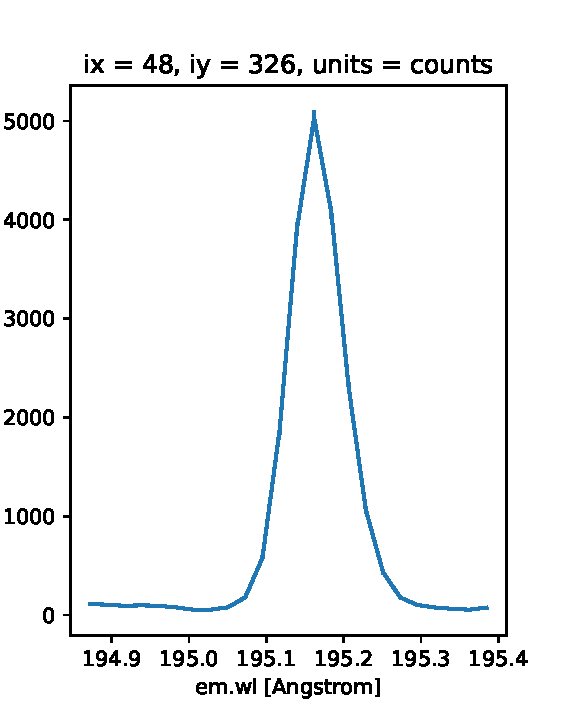
\includegraphics[clip,width=\linewidth]{figures/ex_spectrum.pdf}}
  \caption{An example \ion{Fe}{12} 195.119\,\AA\ line profile from the raster.}
  \label{fig:spectrum}
\end{marginfigure}

The \verb+.plot()+ method can also be used to display the spectrum from a single pixel, as shown
below. For illustration, we also convert the data back in units of photon counts (this is the same as
dividing the calibrated data by the \verb+.meta['radcal']+ array).

\begin{lstlisting}[language=Python]
>>> ix = 48
>>> iy = 326
>>> spec = data_cube[iy,ix,:].remove_radcal()
>>> spec_plot = spec.plot()
>>> spec_plot.set_title(f'ix = {ix}, iy = {iy}, units = counts')
\end{lstlisting}

To perform more advanced plotting, such as logarithmically scaling the intensities, you will need to extract the data from the \verb+EISCube+ and create the figure yourself using any of the various Python plotting libraries. For example,
\begin{marginfigure}
  \centerline{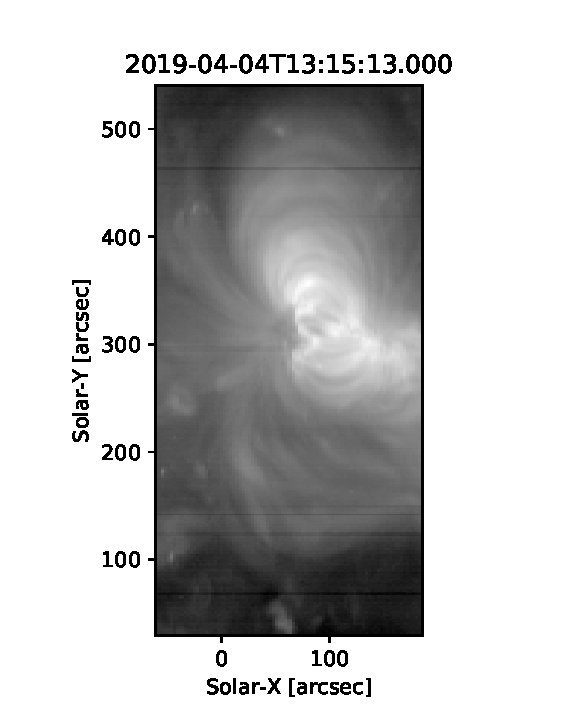
\includegraphics[clip,width=\linewidth]{figures/ex_log-scaled_raster.pdf}}
  \caption{An example image formed by summing the data for the \ion{Fe}{12} spectral window in the
    dispersion direction. In a subsequent chapter we'll discuss fitting the spectra.}
  \label{fig:raster}
\end{marginfigure}
\marginnote{\textbf{Plotting tip:} setting both "aspect" (y\_scale/x\_scale) and "extent" (data range as [left, right, bottom, top]) in \texttt{plt.imshow()} can sometimes give unexpected results. You may need to experiment with the combination of keywords needed to get the plot you expect.}

\begin{lstlisting}[language=Python]
import numpy as np
import matplotlib.pyplot as plt

raster_sum = np.sum(data_cube.data, axis=2) # or data_cube.sum_spectra().data
scaled_img = np.log10(raster_sum)

plt.figure()
plt.imshow(scaled_img, origin='lower', extent=data_cube.meta['extent_arcsec'], cmap='gray')
plt.title(data_cube.meta['date_obs'][-1])
plt.xlabel('Solar-X [arcsec]')
plt.ylabel('Solar-Y [arcsec]')
plt.show()
\end{lstlisting}

We usually don't care about the numbering of the data windows. It's more natural to want to read
the data corresponding to a particular wavelength. The \verb+eispac.read_wininfo()+ function can be used help identify the spectral contents of each data window. The function takes an input header file and returns a record array containing the window numbers, min and max wavelengths and primary spectral line for each data window. Note: for your convenience, a copy of the \verb+wininfo+ array is also stored in the \verb+EISCube.meta+ dictionary.
\begin{lstlisting}[language=Python]
>>> import eispac
>>> header_filename = 'eis_20190404_131513.head.h5'
>>> wininfo = eispac.read_wininfo(header_filename, 195.12)
>>> wininfo.dtype.names
('iwin', 'line_id', 'wvl_min', 'wvl_max', 'nl', 'xs')
>>> wininfo[0:4]
rec.array([(0, 'Fe XI 180.400', 180.03426, 180.72559, 32, 661),
           (1, 'Ca XV 182.100', 181.75139, 182.44266, 32, 738),
           (2, 'Fe X 184.720', 183.82512, 185.5865 , 80, 831),
           (3, 'Fe XII 186.750', 186.3891 , 187.0802 , 32, 946)],
          dtype=[('iwin', '<i4'), ('line_id', '<U64'), ('wvl_min', '<f4'),
                 ('wvl_max', '<f4'), ('nl', '<i4'), ('xs', '<i4')])
\end{lstlisting}
We can then use a numpy.where() call on the wininfo array to map wavelength to window number.
Users familiar with IDL may be interested to note that numpy record arrays can be accessed similarly to an IDL array of structures (e.g. instead of \verb+wininfo['wvl_min']+ below, you could also use \verb+wininfo.wvl_min+).
\begin{lstlisting}
>>> import numpy as np
>>> wvl = 195.119
>>> p = (wininfo['wvl_max'] - wvl)*(wvl - wininfo['wvl_min'])
>>> iwin = np.where(p >= 0)[0]
>>> iwin
array([7], dtype=int64)
\end{lstlisting}
If the result is an empty array, the wavelength is not in the data.


\chapter{Fitting the Data}

Fitting of the spectra involves selecting a spectral line of interest (e.g. \ion{Fe}{12} 195.12\,\AA)
from one of the spectral windows of in the data, choosing a function (or combination of functions) to
fit, and determining an initial guess for each parameter. The next ingredient for a fit is the
selection of an optimization method. By default, EISPAC uses a Python implementation of the well-known
IDL method \textbf{MPFIT}, which solves the non-linear least squares problem using the Levenberg-
Marquardt algorithm. The Python module, \verb+mpfit.py+, can be found on GitHub\sidenote{\url{https://github.com/segasai/astrolibpy/}} and is included in EISPAC. Future versions of the code will include
full support for other fitting packages such as the newer astropy.modeling framework\sidenote{We have
 chosen to use MPFIT due to its flexibility and long (20+ year) legacy in solar and heliophysics. While
 newer fitting methods provide powerful tools for data exploration, they are still young and incur
 significant additional computation time (and are also more complicated to parallelize).}.

\section{Template files}
In order to make fitting quick and easy, we've created a set of fit templates for different spectral lines. An \verb+h5dump+\sidenote{\texttt{h5dump} is a command line tool used to inspect the contents of an HDF5 file. It is included  the Anaconda Python distribution platform, but can also be installed on its own.} on one of the template files shows that it contains a \verb+/template+ group for the initial guess on the fit parameters and a \verb+/parinfo+ group containing constraints on the parameters for use by \verb+mpfit.py+.

\begin{lstlisting}
h5dump -n fe_12_195_119.2c.template.h5
HDF5 "fe_12_195_119.2c.template.h5" {
FILE_CONTENTS {
 group      /
 group      /parinfo
 dataset    /parinfo/fixed
 dataset    /parinfo/limited
 dataset    /parinfo/limits
 dataset    /parinfo/tied
 dataset    /parinfo/value
 group      /template
 dataset    /template/component
 dataset    /template/data_e
 dataset    /template/data_x
 dataset    /template/data_y
 dataset    /template/fit
 dataset    /template/fit_back
 dataset    /template/fit_gauss
 dataset    /template/line_ids
 dataset    /template/n_gauss
 dataset    /template/n_poly
 dataset    /template/order
 dataset    /template/wmax
 dataset    /template/wmin
 }
\end{lstlisting}

The templates files are named according to the following pattern: \verb+{primary spectral line}.{number of Gaussians}c.template.h5+. The function \verb+eispac.read_template()+ can be used to read a template file and examine the contents.

\begin{lstlisting}[language=Python]
>>> import eispac
>>> tmplt_filename = 'fe_12_195_119.2c.template.h5'
>>> tmplt = eispac.read_template(tmplt_filename)
\end{lstlisting}

This produces the output below, which automatically calls the method \verb+.print_parinfo()+ to view the initial parameter values and constraints in a nice format (you can turn off the extra output by setting \verb+quiet=True+).

\begin{lstlisting}
Template file,
   ... fe_12_195_119.2c.template.h5
--- FIT TEMPLATE PARAMETER CONSTRAINTS ---
 *         Value      Fixed        Limited            Limits               Tied
p[0]     57514.6647     0          1    0       0.0000       0.0000
p[1]       195.1179     0          1    1     195.0778     195.1581
p[2]         0.0289     0          1    1       0.0191       0.0510
p[3]      8013.4013     0          1    0       0.0000       0.0000
p[4]       195.1779     0          1    1     195.1378     195.2181          p[1]+0.06
p[5]         0.0289     0          1    1       0.0191       0.0510          p[2]
p[6]       664.3349     0          0    0       0.0000       0.0000
\end{lstlisting}

The structure of \verb+parinfo+ is specific to MPFIT and should be familiar to 
anyone who has used the original IDL version; please see the 
\hyperref[sec:parinfo]{Appendix A} for more details\sidenote{The 
  \texttt{EISFitTemplate} object returned by \texttt{eispac.read\_template} also
  generates a \texttt{.funcinfo} list. This list will help with the implementation
  of other fitting methods in the future, but is currently not used by the code 
  and can, thereby, be safely ignored.}. The templates provided with EISPAC 
consist of one or more Gaussian functions (with parameters in the order of peak,
centroid, \& width) followed by one or more background polynomial terms (usually
just a single, constant value). The values \verb+.template['n_gauss']+ and 
\verb+.template['n_poly']+ indicate, respectively, the number of Gaussian 
functions and background polynomial terms in a given template.

\section{Fitting spectra}
Once you've read in a template file, you can use the central wavelength to find the desired spectral window in the data using \verb+eispac.read_cube()+.\marginnote{\textbf{Reminder:} The command line script \texttt{eis\_fit\_files} can be used to quickly fit a directory of files using one or more templates in another directory.}

\begin{lstlisting}[language=Python]
>>> data_filename = 'eis_20190404_131513.data.h5'
>>> data_cube = eispac.read_cube(data_filename, tmplt.central_wave)
\end{lstlisting}

As mentioned in the previous chapter, \verb+read_cube()+ automatically applies all of the pointing and wavelength corrections, bad data masking, and error estimations needed for scientific analysis. By default, the code also converts the data from photon counts to intensity units of erg cm$^{-2}$ s$^{-1}$ sr$^{-1}$ using the appropraite pre-flight calibration curve. This conversion can be disabled by setting the keyword \verb+apply_radcal=False+, should you prefer to run your fits in count space.

On to the fitting! Now that you have a template and the data elements, you can 
perform a fit of the entire data cube by calling the top-level fitting routine, 
\verb+eispac.fit_spectra()+\sidenote{Here's what's happening under the hood, 
\texttt{fit\_spectra()} calls the helper function \texttt{scale\_guess()} to scale the
initial parameter values to the data, then \texttt{mpfit} is called to actually 
run the Levenberg-Marquardt fitting on a custom function that computes the 
deviates between the input spectrum and a multigaussian fit}. The easiest way to
use \verb+fit_spectra()+ is to just give it both an \verb+EISCube+ and 
\verb+EISFitTemplate+ object (or filepaths to the data and template HDF5 files).
You may slice your \verb+EISCube+ how ever you wish before fitting and the code 
will loop over the data appropriately (this includes fitting a single spectra or
slit observation). Additionally, \verb+fit_spectra()+ takes advantage of the 
\verb+multiprocessing+ package in the Python standard library to automatically 
parallelize the fitting process and minimize the run time. You may control the 
number of processing cores used for the fitting with \verb+ncpu+ keyword, or set
it equal to "max" or None to use the maximum number of cores 
available\sidenote{\textbf{IMPORTANT:} due to the specifics of how the 
multiprocessing library works, any statements that call \texttt{fit\_spectra()} 
using ncpu > 1 MUST be wrapped in a \texttt{"if \_\_name\_\_ == \_\_main\_\_:"} 
statement in the top-level script or program. If such a "name guard" statement 
is not detected, \texttt{fit\_spectra()} will fall back to using a single 
process. Unfortunately, this means you can not directly use parallel fitting 
from an interactive Python shell, you must first write a program that you save 
and run.}.

Here is a minimal example program that just loads and fits the data.
\begin{lstlisting}[language=Python]
import matplotlib.pyplot as plt
import astropy.units as u
import eispac

if __name__ == '__main__':
    # input data and template files
    data_filepath = './eis_20190404_131513.data.h5'
    template_filepath = './fe_12_195_119.2c.template.h5'

    # read fit template
    tmplt = eispac.read_template(template_filepath)

    # Read spectral window into an EISCube
    data_cube = eispac.read_cube(data_filepath, tmplt.central_wave)

    # Fit the data, then save it to disk and test loading it back in
    fit_res = eispac.fit_spectra(data_cube, tmplt, ncpu='max')
    save_filepaths = eispac.save_fit(fit_res, save_dir='cwd')
    load_fit = eispac.read_fit(save_filepaths[0])
\end{lstlisting}

\verb+fit_spectra()+ outputs a \verb+EISFitResult+ object, which may be saved to and HDF5 file and read back in later using the \verb+eispac.save_fit()+ and \verb+eispac.read_fit()+ functions (as shown above). The full doc string for \verb+fit_spectra()+ can be found in \hyperref[sec:fitspec]{Appendix B}

The output fit parameters are stored in a dictionary of arrays.

\begin{lstlisting}[language=Python]
>>> for key in fit_res.fit.keys():
...     print(key, fit_res.fit[key].dtype, fit_res.fit[key].shape)

line_ids <U14 (2,)
main_component int16 ()
n_gauss int16 ()
n_poly int16 ()
status float64 (126, 41)
chi2 float64 (126, 41)
wavelength float64 (126, 41, 24)
int float64 (126, 41, 2)
err_int float64 (126, 41, 2)
params float64 (126, 41, 7)
perror float64 (126, 41, 7)
component int32 (7,)
param_names <U32 (7,)
\end{lstlisting}

The \verb+EISFitResult+ object also has a few methods that make it easy to extract the fit parameters and compute the fit profiles. The use of these methods are demonstrated in the longer example program below, which also shows one way to select a data cutout. Please see \hyperref[sec:EISFitResult]{Appendix B} for more details about the \verb+EISFitResult+ methods.

\begin{lstlisting}[language=Python]
import matplotlib.pyplot as plt
import astropy.units as u
import eispac

if __name__ == '__main__':
    # Read in the fit template and EIS observation
    data_filepath = './eis_20190404_131513.data.h5'
    template_filepath = './fe_12_195_119.2c.template.h5'
    tmplt = eispac.read_template(template_filepath)
    data_cube = eispac.read_cube(data_filepath, tmplt.central_wave)

    # Select a cutout of the raster (note the order of array & plot indices!)
    cutout_extent = [48, 165, 254, 378] # units of [arcsec]
    w_coords = data_cube.axis_world_coords('em.wl')
    lower_left = (cutout_extent[2]*u.arcsec, cutout_extent[0]*u.arcsec,         
                  w_coords[0])
    upper_right = (cutout_extent[3]*u.arcsec, cutout_extent[1]*u.arcsec, 
                   w_coords[-1])
    raster_cutout = data_cube.crop_by_coords(lower_left, 
                                             upper_corner=upper_right)

    # Fit the data and save it to disk
    fit_res = eispac.fit_spectra(raster_cutout, tmplt, ncpu='max')
    save_filepaths = eispac.save_fit(fit_res, save_dir='cwd')

    # Extract array of total data and fit intensites
    sum_data_inten = raster_cutout.sum_spectra().data
    fit_wave_cube, fit_inten_cube = fit_res.get_fit_profile(component=[0,1])
    sum_fit_inten = fit_inten_cube.sum(axis=2)

    # Extract example fit profiles at a higher spectral resolution
    ex_coords = [43, 28] # [Y,X] array coords in units of [pixels]
    fit_x, fit_y = fit_res.get_fit_profile(coords=ex_coords, 
                                           num_wavelengths=100)
    c0_fit_x, c0_fit_y = fit_res.get_fit_profile(component=0, 
                                     coords=ex_coords, num_wavelengths=100)
    c1_fit_x, c1_fit_y = fit_res.get_fit_profile(component=1,
                                     coords=ex_coords, num_wavelengths=100)
    c2_fit_x, c2_fit_y = fit_res.get_fit_profile(component=2,
                                     coords=ex_coords, num_wavelengths=100)
    sub_data = raster_cutout.data[ex_coords[0], ex_coords[1], :]
    sub_wave = raster_cutout.wavelength[ex_coords[0], ex_coords[1], :]
    sub_err = raster_cutout.uncertainty.array[ex_coords[0], ex_coords[1], :]

    # Make a multi-panel figure with the cutout and example
    fig = plt.figure()
    plot_grid = fig.add_gridspec(nrows=2, ncols=2, hspace=0.5, wspace=0.3)

    data_img = fig.add_subplot(plot_grid[0,0])
    data_img.imshow(sum_data_inten, origin='lower', extent=cutout_extent, 
                       cmap='gray')
    data_img.set_title('Data Cutout')
    data_img.set_xlabel('Solar-X [arcsec]')
    data_img.set_ylabel('Solar-Y [arcsec]')

    fit_img = fig.add_subplot(plot_grid[0,1])
    fit_img.imshow(sum_fit_inten, origin='lower', extent=cutout_extent, 
                      cmap='gray')
    fit_img.set_title('Total Fit Intensity')
    fit_img.set_xlabel('Solar-X [arcsec]')
    fit_img.set_ylabel('Solar-Y [arcsec]')

    profile = fig.add_subplot(plot_grid[1,:])
    profile.errorbar(sub_wave, sub_data, yerr=sub_err,
                           ls='', marker='o', color='k')
    profile.plot(fit_x, fit_y, color='b', label='Combined profile')
    profile.plot(c0_fit_x, c0_fit_y, color='r', label='Gaussian 1')
    profile.plot(c1_fit_x, c1_fit_y, color='r', ls='--', label='Gaussian 2')
    profile.plot(c2_fit_x, c2_fit_y, color='g', label='Background')
    profile.set_title(f'Cutout indices iy = {ex_coords[0]},'
                            +f' ix = {ex_coords[1]}')
    profile.set_xlabel('Wavelength [$\AA$]')
    profile.set_ylabel('Intensity ['+str(raster_cutout.unit)+']')
    profile.legend(loc='upper left')
    plt.show()
\end{lstlisting}
\begin{figure}[b!]
  \centerline{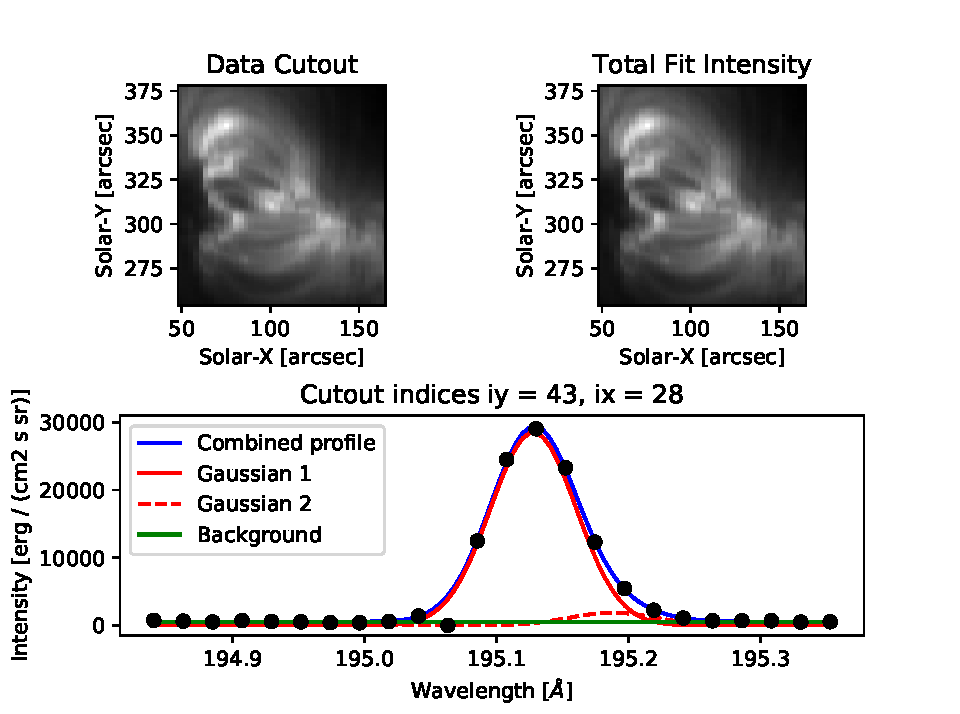
\includegraphics[clip,width=\linewidth]{figures/ex_cutout_and_fit.pdf}}
  \caption{Example data cutout and profile fits. The top two panels show the raster formed by summing
    over the wavelength axis on the observed intensities (left) and fit intensities (right).
    The bottom panel shows an example fit for the \ion{Fe}{12} 195.119\,\AA\ line profile.}
  \label{fig:fit_example}
\end{figure}

\chapter{Level-1 HDF5 File Details}
\label{sec:prep}

This chapter describes in more detail how the EIS level-1 HDF5 files were processed and saved. These HDF5 files can be downloaded from \url{https://eis.nrl.navy.mil/} or by using the search \& download functionality of EISPAC (see \hyperref[sec:download]{Chapter 2}).

\section{Prepping the data in IDL}
The level-0 fits files were prepped using the IDL routine \verb+eis_prep+ available via SolarSoft
\citep{Freeland:1998} with the following options:
\begin{verbatim}
  default = 1
  save = 1
  quiet = 1
  retain = 1
  photons = 1
  refill = 0
\end{verbatim}
There are 400,000+ EIS level-0 files at present, but on a multi-core machine using the IDL bridge
all of the files can be prepped in under 24 hours. We have prepped all of the available EIS files
and saved them to standard fits files in the usual way. Some important points:

\begin{enumerate}
\item[\bf units:] As mentioned previously, the units for the output in these level-1 files is
  ``photon events'' or ``counts.''  This means that the statistical uncertainty can usually be
  estimated as $\sqrt{N}$. When EISPAC loads the HDF5 files, it also calculates an estimate for
  the read noise contribution. It should be noted, however, that the read noise becomes
  significant only at very low flux levels (1--2 counts).

\item[\bf retain:] Note that the retain keyword preserves negative values. One of the jobs of
  \verb+eis_prep+ is to remove the pedestal from the CCD readout and any time-dependent dark
  current. Since the spectral windows are generally narrow, the estimate of the background can be
  too high and the subtracted intensities of the continuum can be negative. This will be dealt with
  during the fitting.

\item[\bf refill:] The warm pixel problem complicates the fitting of EIS line profiles. As
  discussed in the EIS software note \#13 (found in SSW or on the eiswiki), interpolating the values
  of missing pixels appears to best reproduce the original data. This option is left off during
  \verb+eis_prep+ so that the level-1 fits file preserves the information on the missing pixels. As
  discussed below, the interpolation (via the refill option) is done during the read and this data is
  ultimately written to the HDF5 file. A mask indicating which pixels have been interpolated will be
  added to the HDF5 files in a future revision.
\end{enumerate}

Here is an IDL code snippet related to reading the data by looping over the spectral windows.
\begin{lstlisting}[language=idl]
for iwin=0, nwin-1 do begin
  d = eis_getwindata(eis_level1_filename, iwin, /refill, /quiet)
  eis_level1_data[iwin] = ptr_new(d)
endfor
\end{lstlisting}

\section{Writing the HDF5 files}
Each processed level-1 fits file was bundled up with the associated calibration and metadata and saved
as a pair of two HDF5 files:

\begin{enumerate}
\item[\bf eis\_YYYYMMDD\_HHMMSS.data.h5:] Contains only the corrected photon counts within each
  spectral window. This is, by far, the larger of the two HDF5 files. However, they should not need to
  be updated or downloaded very often.
\item[\bf eis\_YYYYMMDD\_HHMMSS.head.h5:] Contains the original fit file index, calibration curves for
  each spectral window (used to convert counts into intensity values), and the corrected pointing
  information.
\end{enumerate}

Users will rarely, if ever, need to access the information inside the HDF5 files directly. EISPAC
contains all of the functions needed to read the data and apply the calibration and pointing
corrections. Nevertheless, the contents and data structure of the HDF5 files are summarized below.

\subsection{.data.h5}
\begin{itemize}
  \item [\bf level1] (group)
  \begin{itemize}
    \item [\bf {intensity\_units}] (dataset) - String with the level1 data units. This will usually be
    "counts"
    \item [\bf {win\#\#}] (dataset) - array of floating point values with the photon counts in a given
    spectral window (e.g. \texttt{win00, win01, ... win24}). Note well, each set of EIS observations may have
    a different number of spectral windows, up to a maximum of 24 windows. Window numbers are
    numbered sequentially from 00; a given wavelength range may be assigned a different window number
    in each EIS study.
  \end{itemize}
\end{itemize}

\subsection{.head.h5}
\begin{itemize}
  \item \textit{Details to be added soon}
\end{itemize}

Additionally, the contents of the HDF5 files can be displayed using
\verb+h5dump+ command line tool, which is provided along with the Anaconda Python distribution
platform or can be installed on its own. Example usage,

\begin{lstlisting}
> h5dump -n eis_20190404_131513.data.h5
FILE_CONTENTS {
group      /
group      /level1
dataset    /level1/intensity_units
dataset    /level1/win00
dataset    /level1/win01
dataset    /level1/win02
dataset    /level1/win03
dataset    /level1/win04
dataset    /level1/win05
. . .
\end{lstlisting}
The actual data associated with each variable can be printed out using the \verb+-d+ option. For
example,
\begin{lstlisting}
> h5dump -d exposure_times/duration eis_20190404_131513.head.h5
HDF5 "eis_20190404_131513.head.h5" {
DATASET "exposure_times/duration" {
   DATATYPE  H5T_IEEE_F32LE
   DATASPACE  SIMPLE { ( 87 ) / ( 87 ) }
   DATA {
   (0): 40.0005, 40.0002, 40.0004, 40.0004, 39.9994, 40.0002, 39.9995, 40,
   (8): 40.0007, 39.9999, 40.0005, 40.0004, 39.9997, 40.0002, 39.9994,
   . . .
}
\end{lstlisting}


\chapter{Acknowledgments}

This work was sponsored by the Chief of Naval Research and NASA's Hinode
project. Hinode is a Japanese mission developed and launched by ISAS/JAXA, with NAOJ as domestic
partner and NASA and STFC (UK) as international partners.


\chapter{Appendix A: mpfit documentation}

\section{parinfo keywords}
\label{sec:parinfo}

\textbf{Constraining Parameter Values with the PARINFO Keyword}

The behavior of MPFIT can be modified with respect to each
parameter to be fitted.  A parameter value can be fixed; simple
boundary constraints can be imposed; limitations on the parameter
changes can be imposed; properties of the automatic derivative can
be modified; and parameters can be tied to one another.

These properties are governed by the PARINFO structure, which is
passed as a keyword parameter to MPFIT.

PARINFO should be a list of dictionaries, one list entry for each parameter.
Each parameter is associated with one element of the array, in
numerical order.  The dictionary can have the following keys
(none are required, keys are case insensitive):

\begin{itemize}

    \item['value' -] the starting parameter value (but see the START\_PARAMS
        parameter for more information).

    \item['fixed' -] a boolean value, whether the parameter is to be held
        fixed or not.  Fixed parameters are not varied by
        MPFIT, but are passed on to MYFUNCT for evaluation.

    \item['limited' -] a two-element boolean array.  If the first/second
        element is set, then the parameter is bounded on the
        lower/upper side.  A parameter can be bounded on both
        sides.  Both LIMITED and LIMITS must be given
        together.

    \item['limits' -] a two-element float array.  Gives the
        parameter limits on the lower and upper sides,
        respectively.  Zero, one or two of these values can be
        set, depending on the values of LIMITED.  Both LIMITED
        and LIMITS must be given together.

    \item['parname' -] a string, giving the name of the parameter.  The
        fitting code of MPFIT does not use this tag in any
        way.  However, the default iterfunct will print the
        parameter name if available.

   \item['step' -] the step size to be used in calculating the numerical
        derivatives.  If set to zero, then the step size is
        computed automatically.  Ignored when AUTODERIVATIVE=0.

    \item['mpside' -] the sidedness of the finite difference when computing
        numerical derivatives.  This field can take four values:
        \begin{itemize}
            \item[0 -] one-sided derivative computed automatically
            \item[1 -] one-sided derivative (f(x+h) - f(x)  )/h
            \item[-1 -] one-sided derivative (f(x)   - f(x-h))/h
            \item[2 -] two-sided derivative (f(x+h) - f(x-h))/(2*h)
        \end{itemize}

        Where "h" is the STEP parameter described above.  The
        "automatic" one-sided derivative method will chose a
        direction for the finite difference which does not
        violate any constraints.  The other methods do not
        perform this check.  The two-sided method is in
        principle more precise, but requires twice as many
        function evaluations.  Default: 0.

    \item['mpmaxstep' -] the maximum change to be made in the parameter
        value.  During the fitting process, the parameter
        will never be changed by more than this value in
        one iteration. A value of 0 indicates no maximum.  Default: 0.

    \item['tied' -] a string expression which "ties" the parameter to other
        free or fixed parameters.  Any expression involving
        constants and the parameter array P are permitted.
        Example: if parameter 2 is always to be twice parameter
        1 then use the following: parinfo(2).tied = '2 * p(1)'.
        Since they are totally constrained, tied parameters are
        considered to be fixed; no errors are computed for them.
        [ NOTE: the PARNAME can't be used in expressions. ]

    \item['mpprint' -] if set to 1, then the default iterfunct will print the
        parameter value.  If set to 0, the parameter value
        will not be printed.  This tag can be used to
        selectively print only a few parameter values out of
        many.  Default: 1 (all parameters printed)
\end{itemize}


\chapter{Appendix B: Useful EISPAC doc strings}

\section{fit\_spectra()}
\label{sec:fitspec}

\begin{lstlisting}[language=Python]
def fit_spectra(inten, template, parinfo=None, wave=None, errs=None,
                min_points=10, ncpu='max', skip_fitting=False):
    """Fit one or more EIS line spectra using mpfit (with multiprocessing).

    Parameters
    ----------
    inten : EISCube object, array_like, or filepath
        One or more intensity profiles to be fit. The code will loop over 
        the data according to its dimensionality. 3D data is assumed to be a 
        full EIS raster (or a sub region), 2D data is assumed to be a single 
        EIS slit, and 1D data is assumed to be a single profile.
    template : EISFitTemplate object, dict, or filepath
        Either an EISFitTemplate, a 'template' dictionary, or the path to a
        template file.
    parinfo : list, optional
        List of dictionaries with fit parameters formatted for use with mpfit.
        Will supercede any parinfo lists loaded from an EISFitTemplate. 
        Required if the 'template' parameter is given as a dictionary.
    wave : array_like, optional
        Associated wavelength values for the spectra. Required if 'inten' is
        given as an array and ignored otherwise.
    errs : array_like, optional
        Intensity error values for the spectra. Required if 'inten' is given 
        as an array and ignored otherwise.
    min_points : int, optional
        Minimum number of good quality data points (i.e. non-zero values & 
        errs) to be used in each fit. Spectra with fewer data points will be 
        skipped. Default is 10.
    ncpu : int, optional
        Number of cpu processes to parallelize over. Must be less than or 
        equal to the total number of cores the system has. If set to 'max' or 
        None, the code will use the maximum number of cores available. 
        Default is 'max'.
        Important: due to the specifics of how the multiprocessing library 
        works, any statements that call fit_spectra() using ncpu > 1 MUST be 
        wrapped in a "if __name__ == __main__:" statement in the top-level 
        program. If such a "name guard" statement is not detected, this 
        function will fall back to using a single process.
    skip_fitting : bool, optional
        If set to True, will skip the fitting altogether and just return an 
        empty EISFitResult instance. Used mainly for testing.

    Returns
    -------
    fit_res : EISFitResult class instance
        An EISFitResult object containing the output fit parameters.
    """
\end{lstlisting}

\section{EISFitResult methods}
\label{sec:EISFitResult}
\begin{lstlisting}[language=Python]
def get_params(self, component=None, param_name=None, coords=None,
               casefold=False):
    """Extract parameters values by component number, name, or pixel coords

    Parameters
    ----------
    component : int or list, optional
        Integer number (or list of ints) of the functional component(s).
        If set to None, will return the total combined fit profile.
        Default is None.
    param_name : str, optional
        String name of the requested parameter. If set to None, will not
        filter based on paramater name. Default is None
    coords : list or tupple, optional
        (Y, X) coordinates of the requested datapoint. If set to None, will
        instead return the parameters at all locations. Default is None
    casefold : bool, optional
        If set to True, will ignore case when extracting parameters by
        name. Default is False.

    Returns
    -------
    param_vals : numpy array
        Parameter values
    param_errs : numpy array
        Estimated parameter errors
    """
\end{lstlisting}

\begin{lstlisting}[language=Python]
def get_fit_profile(self, component=None, coords=None, num_wavelengths=None):
    """Calculate the fit intensity profile (total or component) at a location.

    Parameters
    ----------
    component : int or list, optional
        Integer number (or list of ints) of the functional component(s).
        If set to None, will return the total combined fit profile.
        Default is None.
    coords : list or tupple, optional
        (Y, X) coordinates of the requested datapoint. If set to None, will
        instead return the parameters at all locations. Default is None
    num_wavelengths : int, optional
        Number of wavelength values to compute the fit intensity at. These
        values will be equally spaced and span the entire fit window. If set
        to None, will use the observed wavelength values. Default is None.

    Returns
    -------
    fit_wave : numpy array
        Wavelength values
    fit_inten : numpy array
        Fit intensity values
    """
\end{lstlisting}


\bibliography{eag}
\bibliographystyle{apj}

\end{document}
